\begin{figure}
\centering
\resizebox{\columnwidth}{!}{
\setlength{\figheight}{0.25\textheight}
\begin{tabular}{@{}c c c@{}}
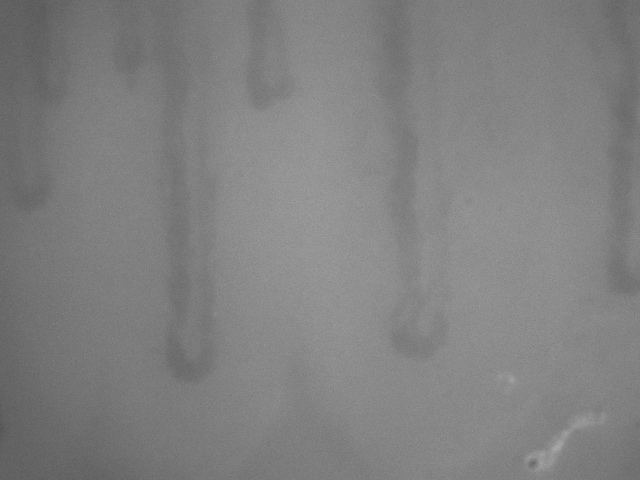
\includegraphics[height=\figheight]{\figpath/real_frame} &
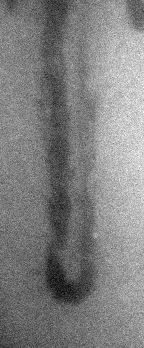
\includegraphics[height=\figheight]{\figpath/real_cap_eq} &
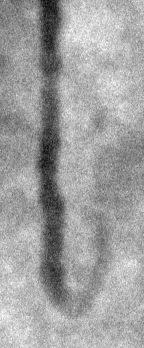
\includegraphics[height=\figheight]{\figpath/fake_cap_eq} \\
(a) & (b) & (c)
\end{tabular}}
%
\caption{Capillaroscopy images: %
(a) Frame from a real capillaroscopy sequence%
%, overlaid with vertical component of estimated blood flow%
; (b) capillary loop from the sequence%
; (c) synthetic capillary generated by our system.
The capillary loops in (b) and (c) have been rescaled to enhance contrast.}
\label{fig_example_images}
\end{figure}
